% Compile with:
% latexmk -lualatex -pvc -interaction=nonstopmode 20220629_MICResearchDay.tex
%\documentclass[aspectratio=169,draft]{beamer}
\documentclass[aspectratio=169]{beamer}
\usetheme{UniBern}

\title{Micro-CT Imaging Across Scales and Faculties}
\author{David Haberthür}
\date{June 29, 2022 | \href{https://www.mic.unibe.ch/events/mic_research_day_2022}{MIC Research Day 2022}}

%\includeonlyframes{current}
%then....
%\begin{frame}[label=current]
%\end{frame}

\usepackage[detect-all=true,
	binary-units=true,
	per-mode=symbol,
	per-symbol=/]{siunitx}
\usepackage{xspace}
\usepackage{gitinfo2}
\usepackage[backend=biber,
	style=numeric,
	url=false,
	maxnames=1,
	sorting=none,
	]{biblatex}
\addbibresource{/Users/habi/Documents/library.bib} % anomalocaris
\addbibresource{/home/habi/P/Documents/library.bib} % anaklin25
\usepackage{ccicons}
\usepackage{animate}
\usepackage{tikz}
	\usetikzlibrary{shadows,spy,mindmap}
	\tikzset{shadowed/.style={preaction={transform canvas={shift={(1pt,-1pt)}},draw=ubRed}}}
\usepackage{shadowtext} % for the shadowed scalebar
	\shadowoffset{1pt}
	\shadowcolor{ubRed}
\usepackage{environ}
\usepackage[absolute,overlay]{textpos} % for the \source* command
\usepackage{fontawesome5}
\usepackage{emoji}
\usepackage{listings}
	\lstset{basicstyle=\tiny\ttfamily}
% highlight a line in listings: https://tex.stackexchange.com/a/58543/828
% Including a crude workaround for recent versions of `listings`: https://tex.stackexchange.com/a/451538/828
\makeatletter
\let\old@lstKV@SwitchCases\lstKV@SwitchCases
\def\lstKV@SwitchCases#1#2#3{}
\makeatother
\usepackage{lstlinebgrd}
\makeatletter
\let\lstKV@SwitchCases\old@lstKV@SwitchCases
\lst@Key{numbers}{none}{%
    \def\lst@PlaceNumber{\lst@linebgrd}%
    \lstKV@SwitchCases{#1}%
    {none:\\%
     left:\def\lst@PlaceNumber{\llap{\normalfont
                \lst@numberstyle{\thelstnumber}\kern\lst@numbersep}\lst@linebgrd}\\%
     right:\def\lst@PlaceNumber{\rlap{\normalfont
                \kern\linewidth \kern\lst@numbersep
                \lst@numberstyle{\thelstnumber}}\lst@linebgrd}%
    }{\PackageError{Listings}{Numbers #1 unknown}\@ehc}}
\makeatother
% highlight a line in listings: https://tex.stackexchange.com/a/58543/828
\usepackage{adjustbox}
\usepackage{microtype}

% Some often used abbreviations/commands
\newcommand{\everyframe}{1} % use only every nth frame for the animations
\newcommand{\imwidth}{\linewidth}% set global image width
\newcommand{\imheight}{0.725\paperheight}% set global image height
\newlength\imagewidth% needed for scalebars
\newlength\imagescale% needed for scalebars
\newcommand{\uct}{\textmu CT\xspace}% make our life easier
\newcommand{\uaf}{\si{\micro}Angiofil\xspace}% make our life easier
\newcommand{\eg}{e.\,g.\xspace}%
\newcommand{\ie}{i.\,e.\xspace}%

% Push content to bottom of page: https://tex.stackexchange.com/a/54237/828
\newcommand{\btVFill}{\vskip0pt plus 1filll}
% and then just add \btVFill whenever needed.

% Acknowledge images just below them
% Based on https://tex.stackexchange.com/a/282637/828
\newcommand{\source}[2]{%
	% Print out (short) link under image, with small text
	\raisebox{-1.618ex}{%
		\makebox[0pt][r]{%
			\scriptsize\href{http://#1}{#1} #2%
			}%
		}%
	}%
\newcommand{\sourcecite}[2]{%
	% Cite (an image from) a reference
	\raisebox{-1.618ex}{%
		\makebox[0pt][r]{%
			\scriptsize From \cite{#1}, #2%
			}%
		}%
	}%
\newcommand{\sourcelink}[3]{%
	% Make the source command an \href{link}{text}
	\raisebox{-1.618ex}{%
		\makebox[0pt][r]{%
			\scriptsize\href{http://#1}{#2}, #3%
			}%
		}%
	}%
% Define us a custom footer *with* progress bar, based on https://tex.stackexchange.com/a/59749/828
\makeatletter
\def\progressbar@progressbar{} % the progress bar
\newcount\progressbar@tmpcounta% auxiliary counter
\newcount\progressbar@tmpcountb% auxiliary counter
\newdimen\progressbar@pbht %progressbar height
\newdimen\progressbar@pbwd %progressbar width
\newdimen\progressbar@rcircle % radius for the circle
\newdimen\progressbar@tmpdim % auxiliary dimension
\progressbar@pbwd=0.8\linewidth
\progressbar@rcircle=1.5pt
\def\progressbar@progressbar{%
	\progressbar@tmpcounta=\insertframenumber
	\progressbar@tmpcountb=\inserttotalframenumber
	\progressbar@tmpdim=\progressbar@pbwd
	\multiply\progressbar@tmpdim by \progressbar@tmpcounta
	\divide\progressbar@tmpdim by \progressbar@tmpcountb
	\par%
	\begin{tikzpicture}%
		\draw[ubGrey] (0,0) -- ++ (\progressbar@pbwd,0);
		\draw[draw=ubRed,fill=ubGrey] (\the\dimexpr\progressbar@tmpdim-\progressbar@rcircle\relax,.5\progressbar@pbht) circle (\progressbar@rcircle);
	\end{tikzpicture}%
	\hfill\xspace|\xspace bit.ly/MICRday\xspace|\xspace%
	v. \href{https://github.com/habi/Talk.2022.MICResearchDay/commit/\gitHash}{\gitAbbrevHash}\xspace|\xspace%
	p.\xspace\insertframenumber/\inserttotalframenumber%
	\hspace*{4ex}%
	\vspace{0.5ex}%
	%\par%
}
\addtobeamertemplate{footline}{}%
{%
	\begin{beamercolorbox}[wd=\paperwidth,center]{ubRed}%
		\progressbar@progressbar%
	\end{beamercolorbox}%
}%
\makeatother

% Format bibliography for beamer
% http://tex.stackexchange.com/a/10686/828
\renewbibmacro{in:}{}
% http://tex.stackexchange.com/a/13076/828
\AtEveryBibitem{%
	\clearfield{journaltitle}
	\clearfield{pages}
	\clearfield{volume}
	\clearfield{number}
	\clearname{editor}
	\clearfield{issn}
	\clearfield{year}
}
% No parentheses around the (now empty) year: https://tex.stackexchange.com/a/147537/828
\renewcommand{\bibopenparen}{\addcomma\addspace}
\renewcommand{\bibcloseparen}{\addcomma\addspace}

% open in fullscreen
%\hypersetup{pdfpagemode=FullScreen}

% Add a sticky note: https://tex.stackexchange.com/a/159690/828
% Download Humor Sans font, too: https://github.com/shreyankg/xkcd-desktop/blob/master/Humor-Sans.ttf
\NewDocumentCommand\StickyNote{O{6cm}mO{6cm}}{%
\begin{tikzpicture}
\node[
draw,
drop shadow={
  shadow xshift=2pt,
  shadow yshift=-4pt
},
inner xsep=7pt,
fill=myyellow,
xslant=-0.1,
yslant=0.1,
inner ysep=10pt
] {\parbox[t][#1][c]{#3}{#2}};
\end{tikzpicture}%
}
\definecolor{myyellow}{RGB}{242,226,149}

% Move the whole text area down a bit
% THIS IS A BIG HACK, AND SHOULD BE FIXED IN THE TEMPLATE
\addtobeamertemplate{frametitle}{}{\vspace*{0.71em}}

\begin{document}
% No footline on the title page
% http://tex.stackexchange.com/a/18829/828 helps us to achieve that
{%
	\setbeamertemplate{footline}{}%
	\begin{frame}%
		\maketitle
	\end{frame}%
}

\begin{frame}
	\frametitle{\emph{Grüessech} from the \uct-group}
	\centering
	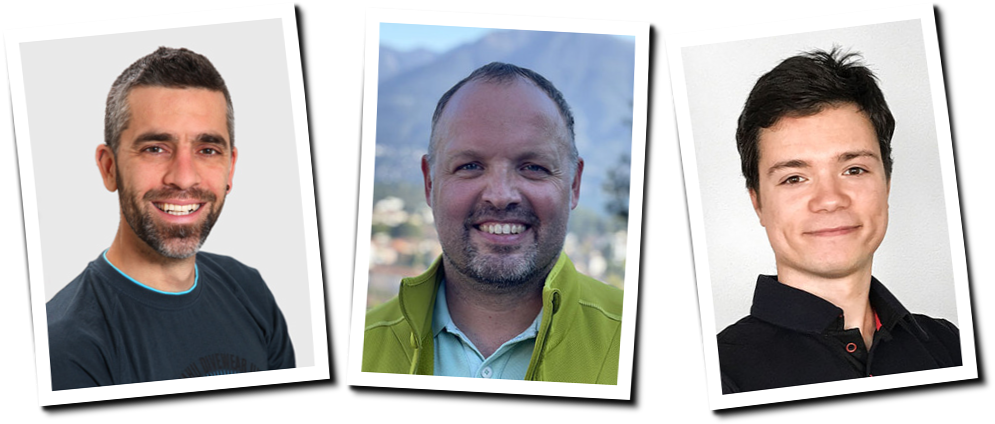
\includegraphics[width=\linewidth]{./images/team}
\end{frame}

%\begin{frame}
%	\frametitle{LOAFS}
%	\uct
%	
%	Non-destructive imaging across scales
%	
%	Ich zeige nur \emph{uni-interne} Projekte, wir machen noch (viel) mehr	
%\end{frame}

\begin{frame}
	\frametitle{Machinery at the Institute of Anatomy}
	\begin{columns}
		\begin{column}{0.33\linewidth}
			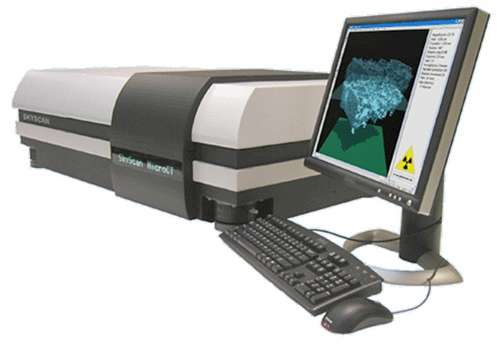
\includegraphics[width=\linewidth]{./images/1172}%
			\source{brukersupport.com}{}
		\end{column}
		\begin{column}{0.33\linewidth}
			\includegraphics<1>[width=\linewidth]{./images/1272}%
			\source{bruker.com/skyscan1272}{}
		\end{column}
		\begin{column}{0.33\linewidth}
			\includegraphics<1>[width=\linewidth]{./images/2214}%
			\source{bruker.com/skyscan2214}{}
		\end{column}							
	\end{columns}
\end{frame}

\begin{frame}
	\frametitle{Overview}
	\centering
	\only<1>{%
		\begin{tikzpicture}%
            \tikzset{small mindmap}%
            \tikzset{level 1 concept/.append style={scale=0.9,level distance = 40mm,transform shape}}%
            \tikzset{level 2 concept/.append style={scale=0.95,level distance = 25mm,transform shape}}%		
		    \path[mindmap,every node/.style={concept,circular drop shadow},concept color=ubRed]%
			    node[concept] {unibe.ch\ Faculties}
			    	child [grow=15]  {node[concept] {Business, Economics ​and Social Sciences}}
    				child [grow=45]  {node[concept] {​Law}}
	    			child [grow=135] {node[concept] {​Human Sciences}}
	       			child [grow=165] {node[concept] {​Science}}
	       			child [grow=195] {node[concept] {​Humanities}}	
	    			child [grow=345] {node[concept] {​Medicine}}
    				child [grow=225] {node[concept] {Vetsuisse}}
	    			child [grow=315] {node[concept] {​Theology}};%
		\end{tikzpicture}%
	}%
	\only<2>{%
		\begin{tikzpicture}%
			\tikzset{small mindmap}%
          		\tikzset{level 1 concept/.append style={scale=0.9,level distance = 40mm,transform shape}}%
			\tikzset{level 2 concept/.append style={scale=0.95,level distance = 25mm,transform shape}}%
		\path[mindmap,every node/.style={concept,circular drop shadow},concept color=ubRed!31!white,semitransparent]%
			node{unibe.ch\ Faculties}
				child [grow=15]  {node[concept] {Business, Economics ​and Social Sciences}}
				child [grow=45]  {node[concept] {​Law}}
				child [grow=135] {node[concept] {​Human Sciences}}
      				child [concept color=ubRed,opaque,grow=165] {node[concept] {Science}}				
    				child [grow=195] {node[concept] {​Humanities}}							
	    			child [concept color=ubRed,opaque,grow=225] {node[concept] {Vetsuisse}}    				
				child [grow=315] {node[concept] {​Theology}}
				child [concept color=ubRed,opaque,grow=345] {node[concept] {​Medicine}};%
		\end{tikzpicture}%
	}%
	\only<3>{%
		\begin{tikzpicture}%
            \tikzset{small mindmap}%
            \tikzset{level 1 concept/.append style={scale=0.9,level distance = 40mm,transform shape}}%
            \tikzset{level 2 concept/.append style={scale=0.95,level distance = 25mm,transform shape}}%		
		    \path[mindmap,every node/.style={concept,circular drop shadow},concept color=ubRed!31!white,semitransparent]%
			    node{unibe.ch\ Faculties}
			    	child [grow=15]  {node[concept] {Business, Economics ​and Social Sciences}}
			    	child [grow=45]  {node[concept] {​Law}}
			    	child [grow=135] {node[concept] {​Human Sciences}}
    		    		child [grow=195] {node[concept] {​Humanities}}
			    	child [grow=315] {node[concept] {​Theology}}
      		    		child [concept color=ubRed,opaque,grow=165] {node[concept] {Science}
			    		child [concept color=ubRed,opaque,grow=-45] {node[concept] {{Institute of Ecology and Evolution}}}
			    		child [concept color=ubRed,opaque,grow=15]  {node[concept] {Space Research \& Planetary Sciences}}
			    		}
    				child [concept color=ubRed,opaque,grow=225] {node[concept] {Vetsuisse}
    				    child [concept color=ubRed,opaque,grow=0] {node[concept] {Clinical radiology}}
    				    }
				    child [concept color=ubRed,opaque,grow=345] {node[concept] {​Medicine}
					    child [concept color=ubRed,opaque,grow=105] {node[concept] {Theodor Kocher Institute}}
    					child [concept color=ubRed,opaque,grow=140] {node[concept] {School of Dental Medicine}}
	    				child [concept color=ubRed,opaque,grow=185] {node[concept] {Institute of Anatomy}}
	    				child [concept color=ubRed,opaque,grow=225] {node[concept] {Klinik für Orthopädische Chirurgie \& Traumatologie}}
	    				};%
		\end{tikzpicture}%
	}%
	% Get emojis from https://unicode.org/emoji/charts/emoji-list.html
	\only<4->{%
		\begin{tikzpicture}%
            \tikzset{small mindmap}%
            \tikzset{level 1 concept/.append style={scale=0.9,level distance = 40mm,transform shape}}%
            \tikzset{level 2 concept/.append style={scale=0.95,level distance = 25mm,transform shape}}%		
		    \path[mindmap,every node/.style={concept,circular drop shadow},concept color=ubRed!31!white,semitransparent]%
			    node{unibe.ch\ Faculties}
			    	child [grow=15]  {node[concept] {Business, Economics ​and Social Sciences}}
			    	child [grow=45]  {node[concept] {​Law}}
			    	child [grow=135] {node[concept] {​Human Sciences}}
    		    		child [grow=195] {node[concept] {​Humanities}}
			    	child [grow=315] {node[concept] {​Theology}}
      		    		child [concept color=ubRed,opaque,grow=165] {node[concept] {Science}
			    		child [concept color=ubRed,opaque,grow=-45] {node[concept] {\huge{\emoji{fish}}}}
			    		child [concept color=ubRed,opaque,grow=15]  {node[concept] {\huge{\emoji{comet}}}}
			    		}
    				child [concept color=ubRed,opaque,grow=225] {node[concept] {Vetsuisse}
    				    child [concept color=ubRed,opaque,grow=0] {node[concept] {\only<4>{\huge{\emoji{unicorn}}}\only<5>{\huge{\emoji{horse}}}}}
    				    }
				    child [concept color=ubRed,opaque,grow=345] {node[concept] {​Medicine}
				    	child [concept color=ubRed,opaque,grow=105] {node[concept] {\huge{\emoji{mouse-face}}}}
    					child [concept color=ubRed,opaque,grow=140] {node[concept] {\huge{\emoji{tooth}}}}
	    				child [concept color=ubRed,opaque,grow=185] {node[concept] {Institute of Anatomy}}
	    				child [concept color=ubRed,opaque,grow=225] {node[concept] {\huge\emoji{bone}}}
					};%
		\end{tikzpicture}%
	}%		
\end{frame}

\begin{frame}
	\frametitle{Hoof}%
	\begin{columns}%
		\begin{column}{0.495\linewidth}%
		\begin{itemize}
			\item Vetsuisse
			\begin{itemize}%
				\item Elke Van der Vekens
			\end{itemize}
			\item Horse hoof
			\item Laminitis \cite{Blaettler2022}, Blood supply%
    			\item Instilled with Angiofil for display of blood vessels
		\end{itemize}
		\end{column}%
		\begin{column}{0.495\linewidth}%
	        \centering%
            \only<1>{%
                \animategraphics[autoplay,height=\imheight,every=\everyframe]{24}{./images/VETSUISSE/HorseLimb/Limb02/setup-frames/IMG_69500}{001}{634}%
                }%
            \only<2>{%
            	\lstinputlisting[linerange={2-4,7-7,15-18,28-29,31-31,36-37,42-42,45-45,55-56},linebackgroundcolor={\ifnum\value{lstnumber}=11\color{ubRed!31}\fi}]{./images/VETSUISSE/HorseLimb/Limb02/proj_01_00mm_41.0um_AlCu/Limb02.log}%
            }%
            \only<3->{%
                \renewcommand{\imwidth}{1.035738368*\imheight}% 1536/1483    
                \pgfmathsetlength{\imagewidth}{\imwidth}%
		        \pgfmathsetlength{\imagescale}{\imagewidth/1536}%
		        \def\x{949-100}% scalebar-x starting at golden ratio of image width of 1536px = 949
		        \def\y{1335}% scalebar-y at 90% of image height of 1483px = 1335
		  	\def\mag{4}% magnification of inset
			\def\size{75}% size of inset
			\begin{tikzpicture}[x=\imagescale,y=-\imagescale,spy using outlines={rectangle,magnification=\mag,size=\size,connect spies}]
			        \node[anchor=north west, inner sep=0pt, outer sep=0pt] at (0,0) {\includegraphics[width=\imagewidth]{./images/VETSUISSE/HorseLimb/Limb02/"MAX_Reslice of merged-bin2x"}};
			        \only<4>{\spy [red] on (468,1252) in node at (768,740) [anchor=center];}
			        % Since we draw the scale bar on the *binned* dataset, each pixel is not 40.999924, but 81.999848 um
			        % 1536.000px = 125.95176652800001mm -> 100px = 8199.985um -> 6.098px = 500um, 1.220px = 100um
			        %draw[|-|,blue,thick] (0,742) -- (1536,742) node [sloped,midway,above,fill=white,semitransparent,text opacity=1] {\SI{125.95}{\milli\meter} (1536px) TEMPORARY!};
			        \draw[|-|,white,thick,shadowed] (\x,\y) -- (\x+609.8,\y) node [midway,above] {\shadowtext{\SI{5}{\centi\meter}}};
		        \end{tikzpicture}%
		        }%
	    \end{column}%
    \end{columns}%
\end{frame}

%Reset image height
\renewcommand{\imheight}{0.725\paperheight}% set global image height
\begin{frame}
	\frametitle{Hoof}
        \centering
		\animategraphics[autoplay,height=\imheight,every=\everyframe]{24}{./images/VETSUISSE/HorseLimb/Limb02/frames/video-0}{000}{300}
\end{frame}

\begin{frame}
	\frametitle{Sacrum}
	\begin{columns}
		\begin{column}{0.495\linewidth}
		\begin{itemize}
			\item Institute of Anatomy and Klinik für Orthopädische Chirurgie \& Traumatologie
			\begin{itemize}%
				\item Sebastian Halm
				\item Johannes D.~Bastian			
			\end{itemize}
			\item Human sacrum
			\item Blood supply
    			\item Instilled with \uaf~\cite{Hlushchuk2018}
		\end{itemize}
		\end{column}
		\begin{column}{0.495\linewidth}
\lstinputlisting[linerange={2-4,7-7,15-18,28-29,31-31,36-37,42-42,45-45,55-56},linebackgroundcolor={\ifnum\value{lstnumber}=11\color{ubRed!31}\fi}]{./images/Halm/Becken/Sakrum_C/proj_047um/SakrumC.log}%
		\end{column}
	\end{columns}
\end{frame}

\begin{frame}
	\frametitle{Sacrum}
		\centering
		\only<1>{%
			\renewcommand{\imwidth}{\imheight}% Fortunately, we have square frames here...
			\pgfmathsetlength{\imagewidth}{\imwidth}%
			\pgfmathsetlength{\imagescale}{\imagewidth/1024}%
			\def\x{633}% scalebar-x starting at golden ratio of image width of 1024px = 633
			\def\y{922}% scalebar-y at 90% of image height of 1024px = 922
			\begin{tikzpicture}[x=\imagescale,y=-\imagescale]
				\node[anchor=north west, inner sep=0pt, outer sep=0pt] at (0,0) {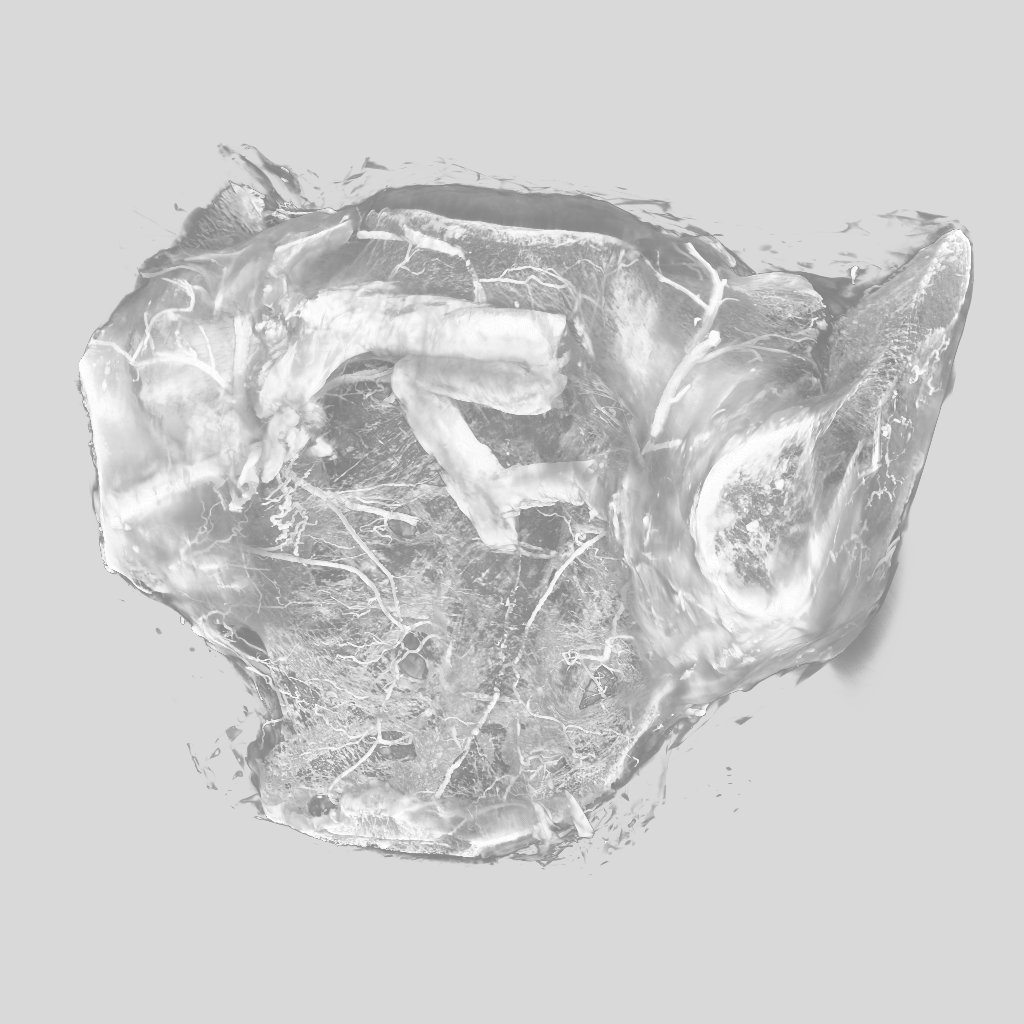
\includegraphics[width=\imagewidth]{./images/Halm/Becken/Sakrum_C/frames/video-0000}};
				% 723.669px = 160.034942115mm -> 100px = 22114.394um -> 2.261px = 500um, 0.452px = 100um
				\draw[|-|,white,thick,shadowed] (77,366) -- (797,436) node [sloped,midway,above] {\shadowtext{\SI{16}{\centi\meter}}};
			\end{tikzpicture}%
			}%
		\only<2>{%
			\animategraphics[autoplay,loop,height=\imheight,every=\everyframe]{24}{./images/Halm/Becken/Sakrum_C/frames/video-0}{000}{300}%
			}%
\end{frame}

% Fishes EAWAG
% Fishec	FieldID	OtherID	ReplacementID	FishID_ColourScanStatus	Length(cm)	TemporaryJar	Genus	Species	Ecology	Replicates
% 103754				103754	6.2		Yssichromis (core)	pyrrhocephalus	zooplanktivore	TZ 2010 MG transect
% 161543				161543 - reconstruct	17	Mark6	Harpagochromis	cf. pachycephalus	piscivore	TZ 2017

\begin{frame}
	\frametitle{Cichlids}
	\begin{columns}
		\begin{column}{0.495\linewidth}
			\begin{itemize}
				\item Institute of Ecology and Evolution
				\begin{itemize}%
					\item Ole Seehausen
					\item Marcel Häsler
					\item Mikki Law
					\item Kassandra Ford
				\end{itemize}
				\item Lake victoria fishes
				\item Morphological description of oral and pharyngeal jaws
    				\item PCA of skull structure
			\end{itemize}
		\end{column}
		\begin{column}{0.495\linewidth}
\lstinputlisting[linerange={2-4,7-7,15-18,28-29,31-31,36-37,42-42,45-45,55-56},linebackgroundcolor={\ifnum\value{lstnumber}=11\color{ubRed!31}\fi}]{./images/EAWAG/161543/head_30um/proj/161543.log}%
		\end{column}
	\end{columns}
\end{frame}

\begin{frame}
	\frametitle{Cichlids}
	       \centering
	       % # Fish 161543, Scan head_30um_rec was scanned with 30 um
	       % 161543 is 17 cm long
	       % For the visualisation, we binned the stack 2x, thus have a voxel size of 60 um
	       % The image is 1412 pixels high, so we used `python ~/P/Dev/latex/draw_a_scalebar.py -p 12 -i frames/video-0000.jpg -l 1412` to draw a scale bar
		\only<1>{%
			\tikzset{shadowed/.style={preaction={transform canvas={shift={(1pt,-1pt)}},draw=ubRed, thick}}} % shadowed drawing https://tex.stackexchange.com/a/185853/828
			\renewcommand{\imwidth}{\imheight/600*1024}%% My script breaks if we have a set image height. The movie frames are 1024x600, so we just calculate a new imwidth :)
			\pgfmathsetlength{\imagewidth}{\imwidth}%
			\pgfmathsetlength{\imagescale}{\imagewidth/1024}%
			\def\x{633-50}% scalebar-x starting at golden ratio of image width of 1024px = 633
			\def\y{540}% scalebar-y at 90% of image height of 600px = 540
			\begin{tikzpicture}[x=\imagescale,y=-\imagescale]
			        \node[anchor=north west, inner sep=0pt, outer sep=0pt] at (0,0) {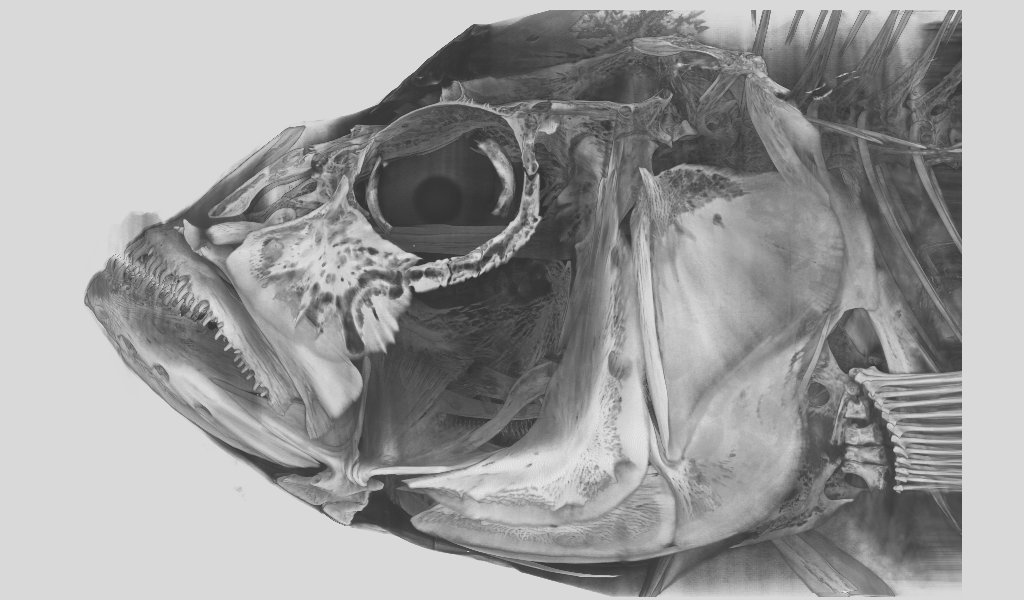
\includegraphics[width=\imagewidth]{./images/EAWAG/161543/head_30um/frames/video-0000}};
			        % 586.337px = 88.08mm -> 100px = 15022.075um -> 3.328px = 500um, 0.666px = 100um
			        %\draw[|-|,blue,thick] (955,6) -- (960,592) node [sloped,midway,above,fill=white,semitransparent,text opacity=1] {\SI{88.08}{\milli\meter} (586px) TEMPORARY!};
			        \draw[|-|,white,thick,shadowed] (\x,\y) -- (\x+332.8,\y) node [midway,above] {\shadowtext{\SI{5}{\centi\meter}}};
		        \end{tikzpicture}%
		        }%
		\only<2>{%
		        \animategraphics[autoplay,height=\imheight,every=\everyframe]{24}{./images/EAWAG/161543/head_30um/frames/video-0}{000}{082}%
	    	}%
		\only<3>{%
		        \animategraphics[autoplay,height=\imheight,every=\everyframe]{24}{./images/EAWAG/161543/head_30um/frames/video-0}{082}{162}%
	    	}%
           	\only<4>{%
		        \animategraphics[autoplay,height=\imheight,every=\everyframe]{24}{./images/EAWAG/161543/head_30um/frames/video-0}{122}{241}%
	    	}%
           	\only<5>{%
		        \animategraphics[autoplay,height=\imheight,every=\everyframe]{24}{./images/EAWAG/161543/head_30um/frames/video-0}{241}{320}%
	    	}%
\end{frame}

\begin{frame}
	\frametitle{Cichlids}
	\begin{columns}
		\begin{column}{0.495\linewidth}
			\begin{itemize}
				\item Institute of Ecology and Evolution
				\begin{itemize}%
					\item Ole Seehausen
					\item Marcel Häsler
					\item Mikki Law
					\item Kassandra Ford
				\end{itemize}
				\item 150 Lake victoria fishes (+300 tomographic scans)
				\item Morphological description of oral and pharyngeal jaws
    				\item PCA of skull structure
			\end{itemize}
		\end{column}
		\begin{column}{0.495\linewidth}
\lstinputlisting[linerange={2-4,7-7,15-18,28-29,31-31,36-37,42-42,45-45,55-56},linebackgroundcolor={\ifnum\value{lstnumber}=11\color{ubRed!31}\fi}]{./images/EAWAG/103754/head/proj/103754.log}%
		\end{column}
	\end{columns}
\end{frame}

\begin{frame}
	\frametitle{Cichlids}
	    \centering
	    % # Fish 103754, Scan head_rec was scanned with 12 um.
	    % 103754 is 6.2 cm long
	    % The image is 1412 pixels high, so we used `python ~/P/Dev/latex/draw_a_scalebar.py -p 12 -i frames/video-0000.jpg -l 1412` to draw a scale bar
\only<1>{%
            \renewcommand{\imwidth}{\imheight/600*1024}%% My script breaks if we have a set image height. The movie frames are 1024x600, so we just calculate a new imwidth :)
	            \tikzset{shadowed/.style={preaction={transform canvas={shift={(1pt,-1pt)}},draw=ubRed, thick}}}% shadowed drawing https://tex.stackexchange.com/a/185853/828
                \pgfmathsetlength{\imagewidth}{\imwidth}%
                \pgfmathsetlength{\imagescale}{\imagewidth/1024}%
                \def\x{633}% scalebar-x starting at golden ratio of image width of 1024px = 633
                \def\y{540}% scalebar-y at 90% of image height of 600px = 540
	            \begin{tikzpicture}[x=\imagescale,y=-\imagescale]
                    	\node[anchor=north west, inner sep=0pt, outer sep=0pt] at (0,0) {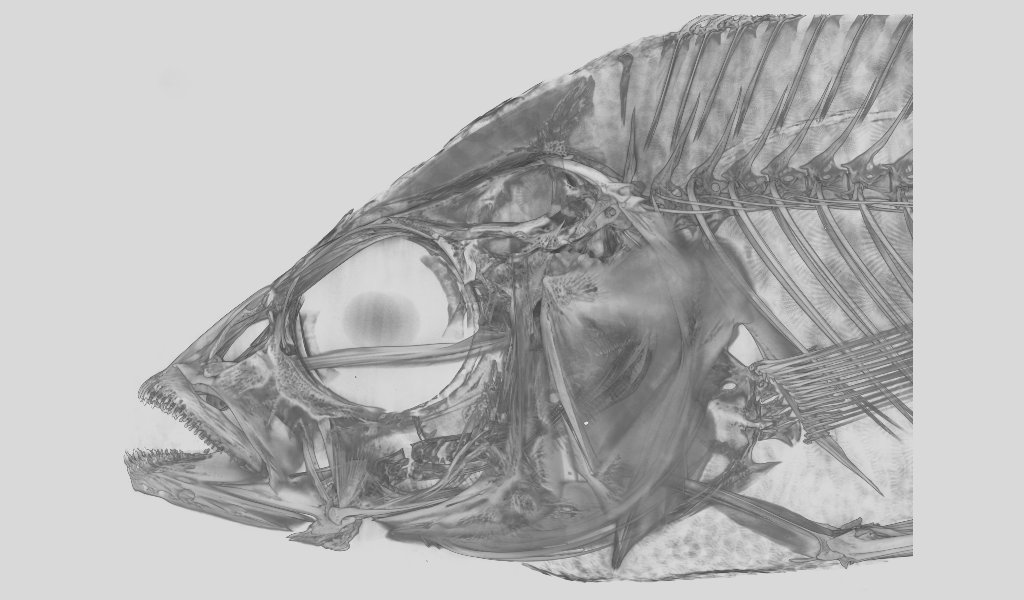
\includegraphics[width=\imagewidth]{./images/EAWAG/103754/head/frames/video-0000}};
                    	% 538.843px = 16.944mm -> 100px = 3144.517um -> 15.901px = 500um, 3.180px = 100um
	               %\draw[|-|,blue,thick] (912,14) -- (910,553) node [sloped,midway,above,fill=white,semitransparent,text opacity=1] {\SI{16.944}{\milli\meter} (539px) TEMPORARY!};
	                \draw[|-|,white,thick,shadowed] (\x,\y) -- (\x+159.01,\y) node [midway,above] {\shadowtext{\SI{500}{\micro\meter}}};
                \end{tikzpicture}%
            }%
	    \only<2>{%
	        \animategraphics[autoplay,height=\imheight,every=\everyframe]{24}{./images/EAWAG/103754/head/frames/video-0}{000}{082}%
	    }%
	    \only<3>{%
	        \animategraphics[autoplay,height=\imheight,every=\everyframe]{24}{./images/EAWAG/103754/head/frames/video-0}{082}{162}%
	    }%
	    \only<4>{%
	        \animategraphics[autoplay,height=\imheight,every=\everyframe]{24}{./images/EAWAG/103754/head/frames/video-0}{162}{241}%
	    }%
	    \only<5>{%
	        \animategraphics[autoplay,height=\imheight,every=\everyframe]{24}{./images/EAWAG/103754/head/frames/video-0}{241}{320}%
	    }%
\end{frame}

\begin{frame}
	\frametitle{Mouse brain vasculature}
	\begin{columns}
		\begin{column}{0.495\linewidth}
			\begin{itemize}
				\item TKI
				\begin{itemize}%
					\item Britta Engelhardt
					\item Kristina Berve
				\end{itemize}
				\item Mouse skulls
				\item Brain vasculature instilled with \uaf~\cite{Hlushchuk2018} 
			\end{itemize}
		\end{column}
		\begin{column}{0.495\linewidth}
\lstinputlisting[linerange={2-5,8-8,21-21,23-23,26-27,24-25,36-36,45-46,41-41,57-58},linebackgroundcolor={\ifnum\value{lstnumber}=11\color{ubRed!31}\fi}]{./images/TKI/TKI_control2_1_65um_al05/proj/TKI_control2_1_65um_al05.log}%
		\end{column}
	\end{columns}
\end{frame}

\begin{frame}
	\frametitle{Mouse brain vasculature}
	% Image Pixel Size (um)=    1.66
	% We used a 2x binned dataset for the visualisation, e.g. the voxel size is 3.32 um
	% The 'length' of the dataset of the skull is 2176 slices, so we used `python ~/P/Dev/latex/draw_a_scalebar.py -p 3.32 -i frames/video-0000.jpg -l 2176` to generate a scale bar for the initial view.
            \renewcommand{\imwidth}{\imheight/600*1024}%% My script breaks if we have a set image height. The movie frames are 1024x600, so we just calculate a new imwidth :)
	          %  \tikzset{shadowed/.style={preaction={transform canvas={shift={(1pt,-1pt)}},draw=ubRed, thick}}}% shadowed drawing https://tex.stackexchange.com/a/185853/828
                \pgfmathsetlength{\imagewidth}{\imwidth}%
                \pgfmathsetlength{\imagescale}{\imagewidth/1024}%
\begin{tikzpicture}[remember picture,overlay]%
		\node at (current page.center) [shift={(0,-25pt)}]{%
			\only<1>{
\def\x{633}% scalebar-x starting at golden ratio of image width of 1024px = 633
\def\y{540}% scalebar-y at 90% of image height of 600px = 540
\begin{tikzpicture}[x=\imagescale,y=-\imagescale]
		\node[anchor=north west, inner sep=0pt, outer sep=0pt] at (0,0) {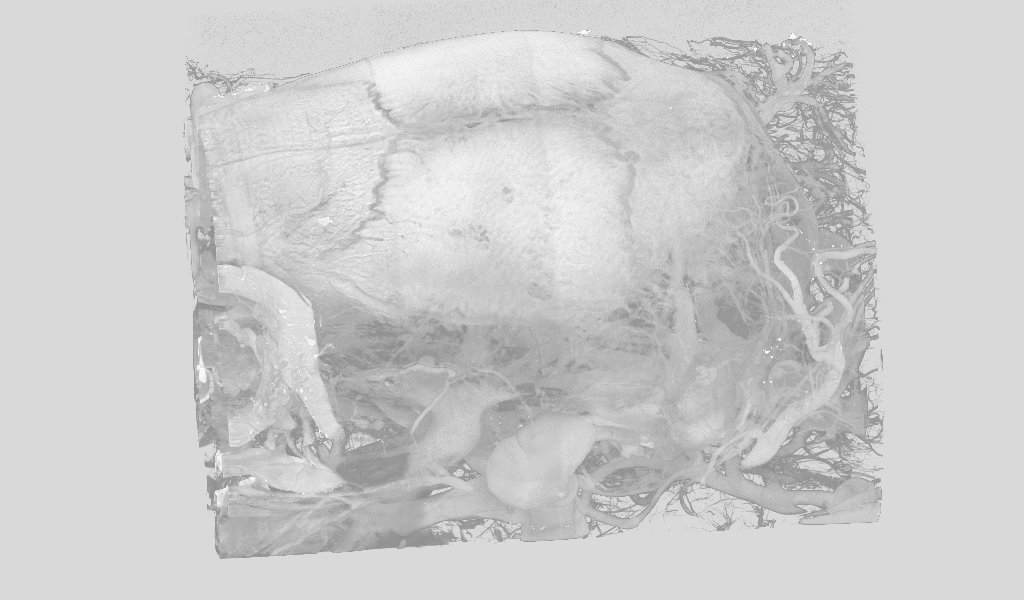
\includegraphics[width=\imagewidth]{./images/TKI/TKI_control2_1_65um_al05/frames/video-0000}};
	% 660.602px = 7.22432mm -> 100px = 1093.597um -> 45.721px = 500um, 9.144px = 100um
	%\draw[|-|,blue,thick] (220,555) -- (880,519) node [sloped,midway,above,fill=white,semitransparent,text opacity=1] {\SI{7.22432}{\milli\meter} (661px) TEMPORARY!};
	\draw[|-|,white,thick,shadowed] (\x,\y) -- (\x+45.721+45.721,\y) node [midway,above] {\shadowtext{\SI{1}{\milli\meter}}};
\end{tikzpicture}%	
			}%
			\only<2>{\animategraphics[autoplay,height=\imheight,every=\everyframe]{24}{./images/TKI/TKI_control2_1_65um_al05/frames/video-0}{000}{100}}%
			\only<3>{\animategraphics[autoplay,height=\imheight,every=\everyframe]{24}{./images/TKI/TKI_control2_1_65um_al05/frames/video-0}{100}{320}}%
			};%
	\end{tikzpicture}%
\end{frame}

\renewcommand{\imwidth}{0.75\linewidth}
\renewcommand{\imheight}{0.618\paperheight}
\begin{frame}
	\frametitle{Teeth}
	\begin{columns}
		\begin{column}{0.495\linewidth}
			\begin{itemize}%
				\item School of Dental Medicine
				\begin{itemize}%
					\item Thomas G.~Wolf
					\item Andrea Anderegg
				\end{itemize}%
				\item 104 human canines
				\item Root canal morphology, according to~\citeauthor{Briseno-Marroquin2015}~\cite{Briseno-Marroquin2015}%
				\item Reproducible analysis~\cite{Haberthur2021}%
			\end{itemize}%
		\end{column}%
		\begin{column}{0.495\linewidth}
			\only<1>{%
				\centering%
				\pgfmathsetlength{\imagewidth}{\imwidth}%
				\pgfmathsetlength{\imagescale}{\imagewidth/2716}%
				\def\x{1678}% scalebar-x starting at golden ratio of image width of 2716px = 1678
				\def\y{2444}% scalebar-y at 90% of image height of 2716px = 2444
				\begin{tikzpicture}[x=\imagescale,y=-\imagescale]%
					\node[anchor=north west, inner sep=0pt, outer sep=0pt] at (0,0) {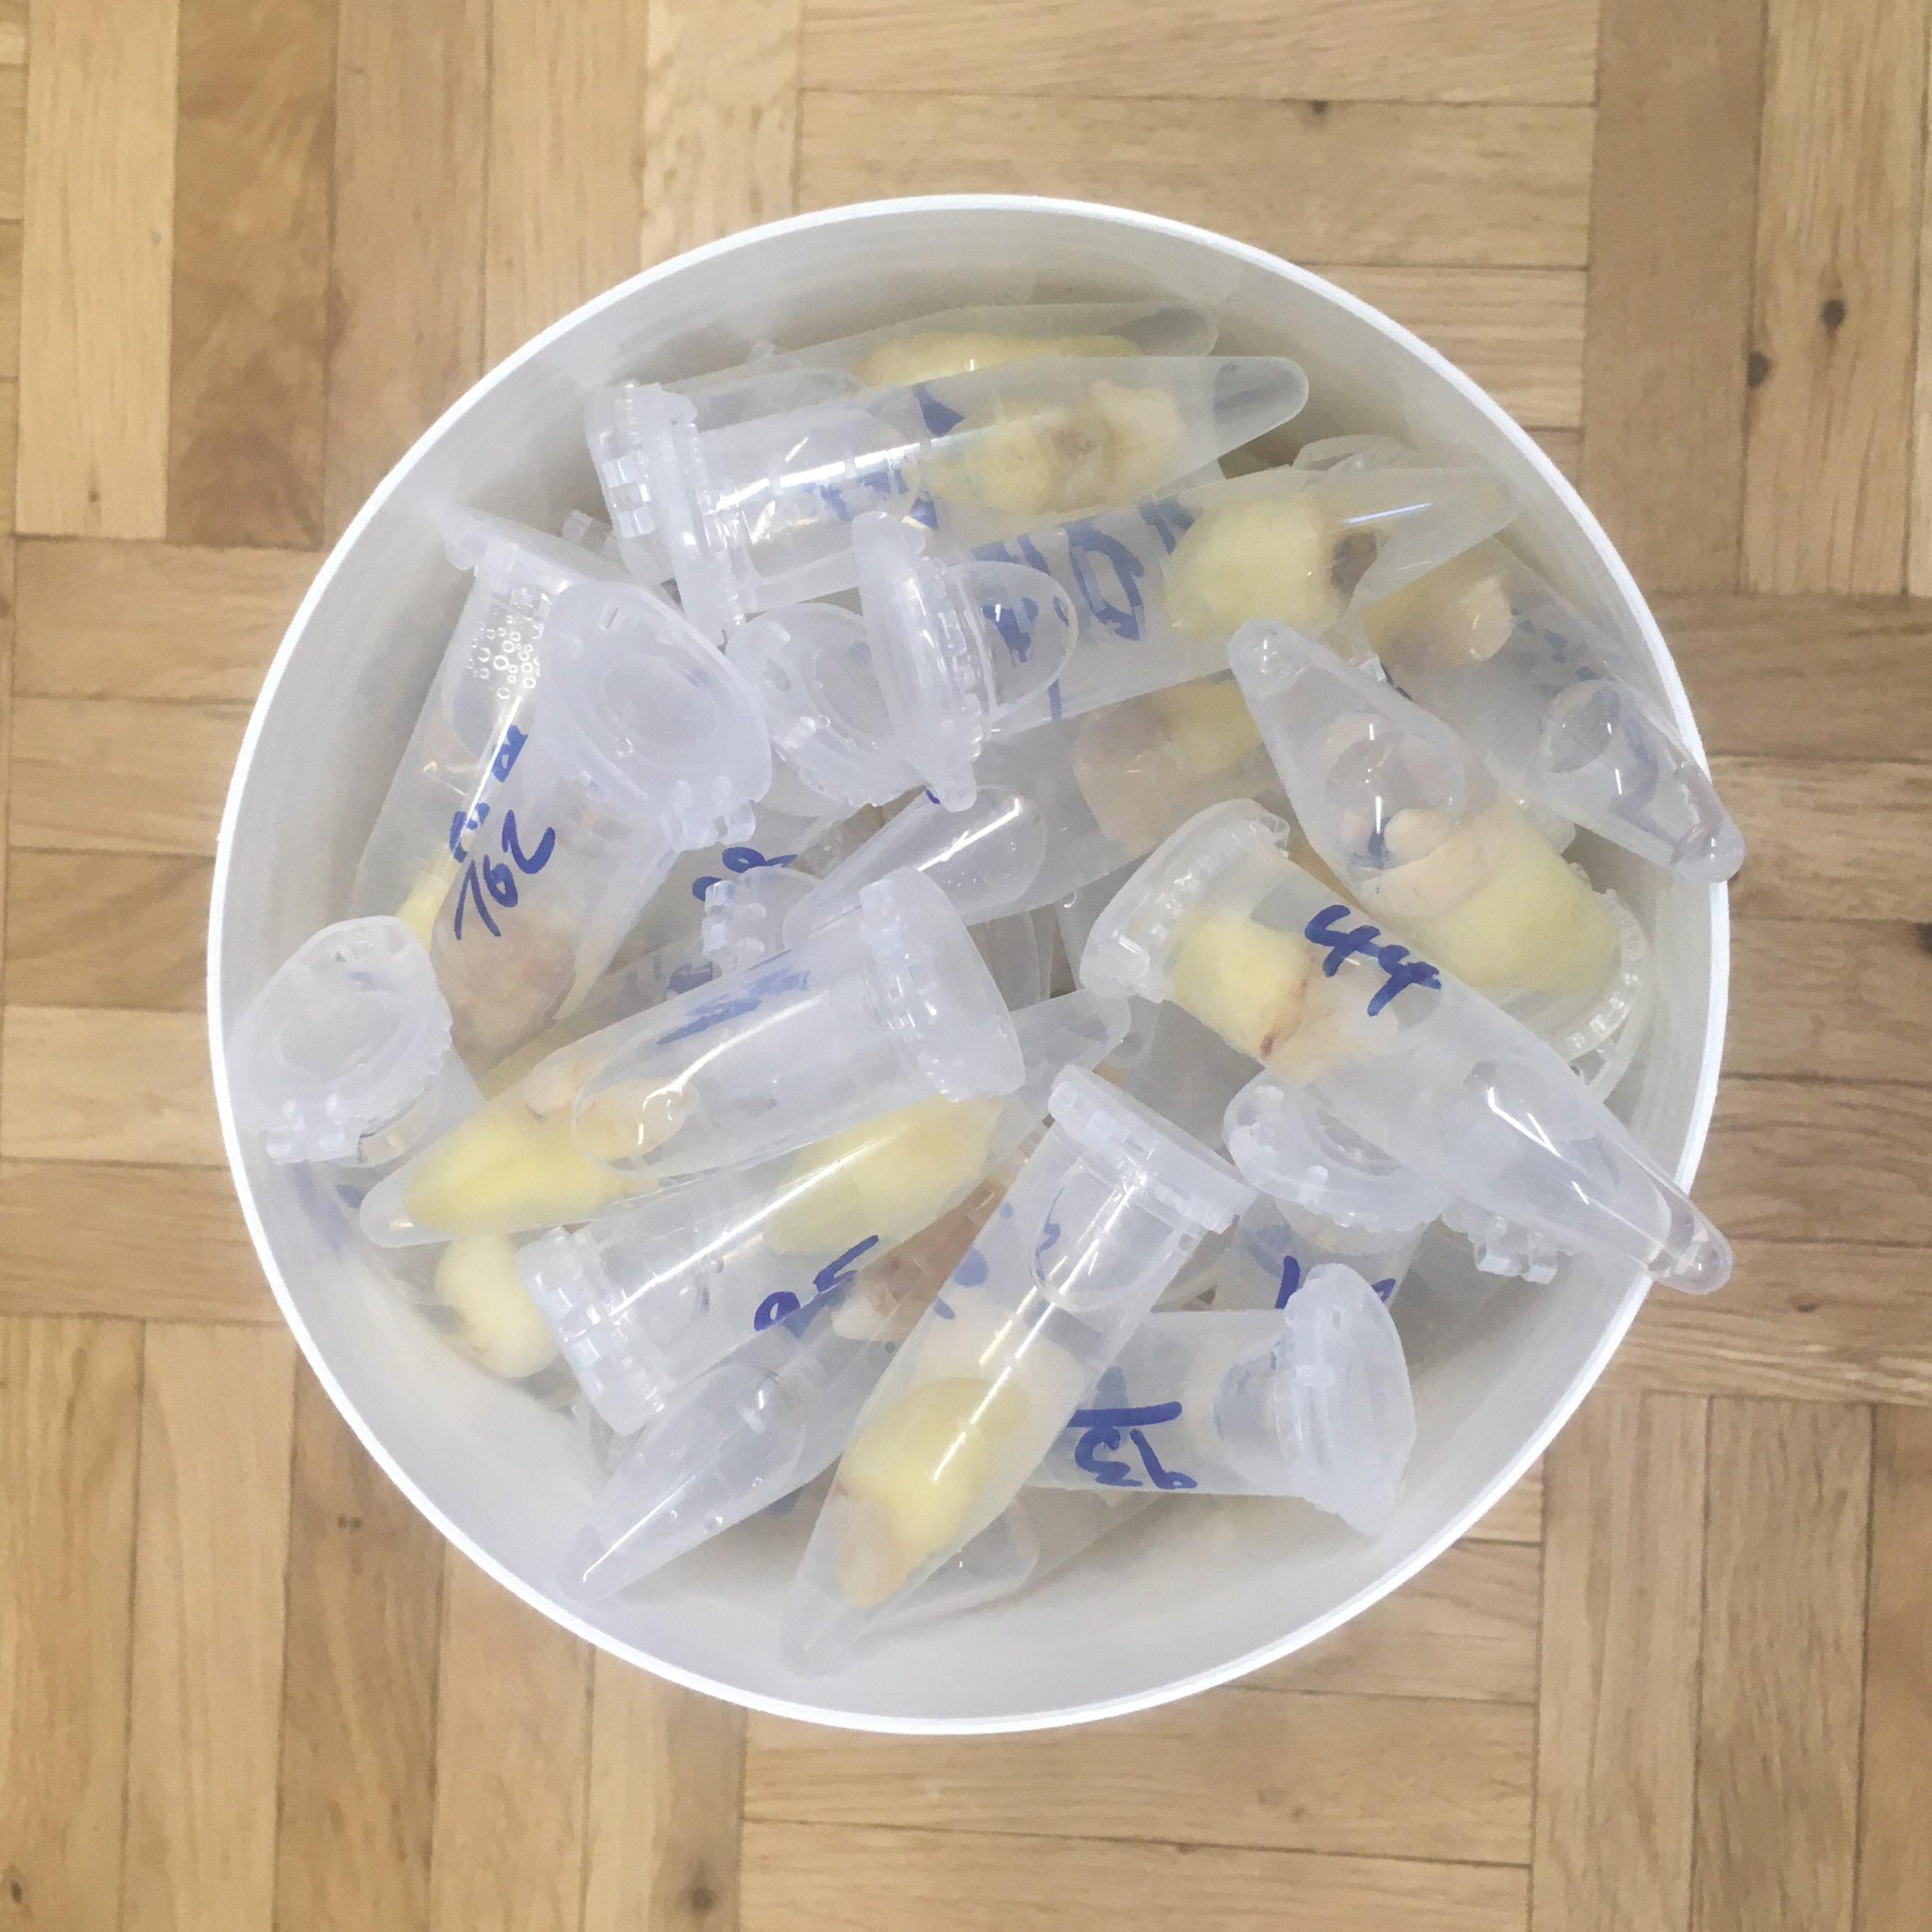
\includegraphics[width=\imagewidth]{./images/ZMK/bucketofteeth}};
					% 2132.087px = 140.0mm -> 100px = 6566.337um -> 7.615px = 500um, 1.523px = 100um
					\draw[|-|,white,thick,shadowed] (\x,\y) -- (\x+761.5,\y) node [midway,above] {\shadowtext{\SI{5}{\centi\meter}}};
				\end{tikzpicture}%
				}%
			\only<2>{%
				\lstinputlisting[linerange={2-4,15-15,17-19,28-30,36-37,40-40,44-44,53-54},linebackgroundcolor={\ifnum\value{lstnumber}=10\color{ubRed!31}\fi}]{./images/ZMK/45/proj/Tooth045.log}%
			}%
			\renewcommand{\imwidth}{\linewidth}%
			\only<3>{%
				\centering%
				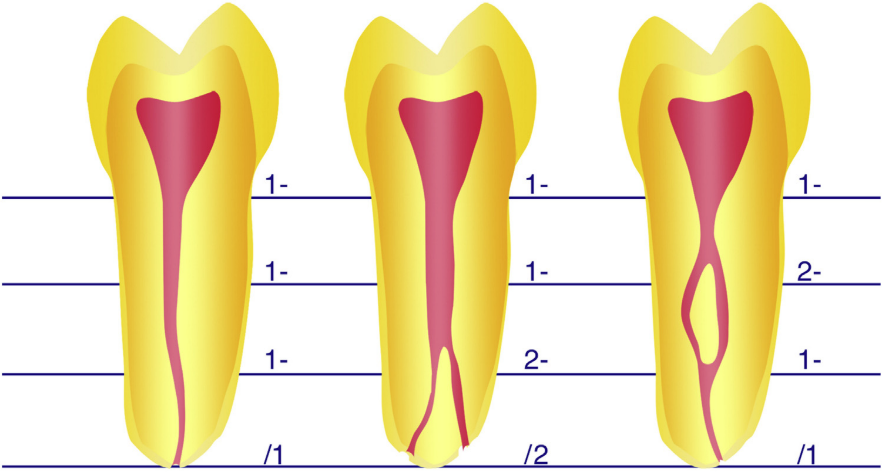
\includegraphics[width=\imwidth]{./images/ZMK/briseno}%
				\sourcecite{Briseno-Marroquin2015}{Fig.~2}%
				}%
			\only<4>{%
				\centering%
				\href{https://mybinder.org/v2/gh/habi/zmk-tooth-cohort/master?filepath=ToothAnalysis.ipynb}{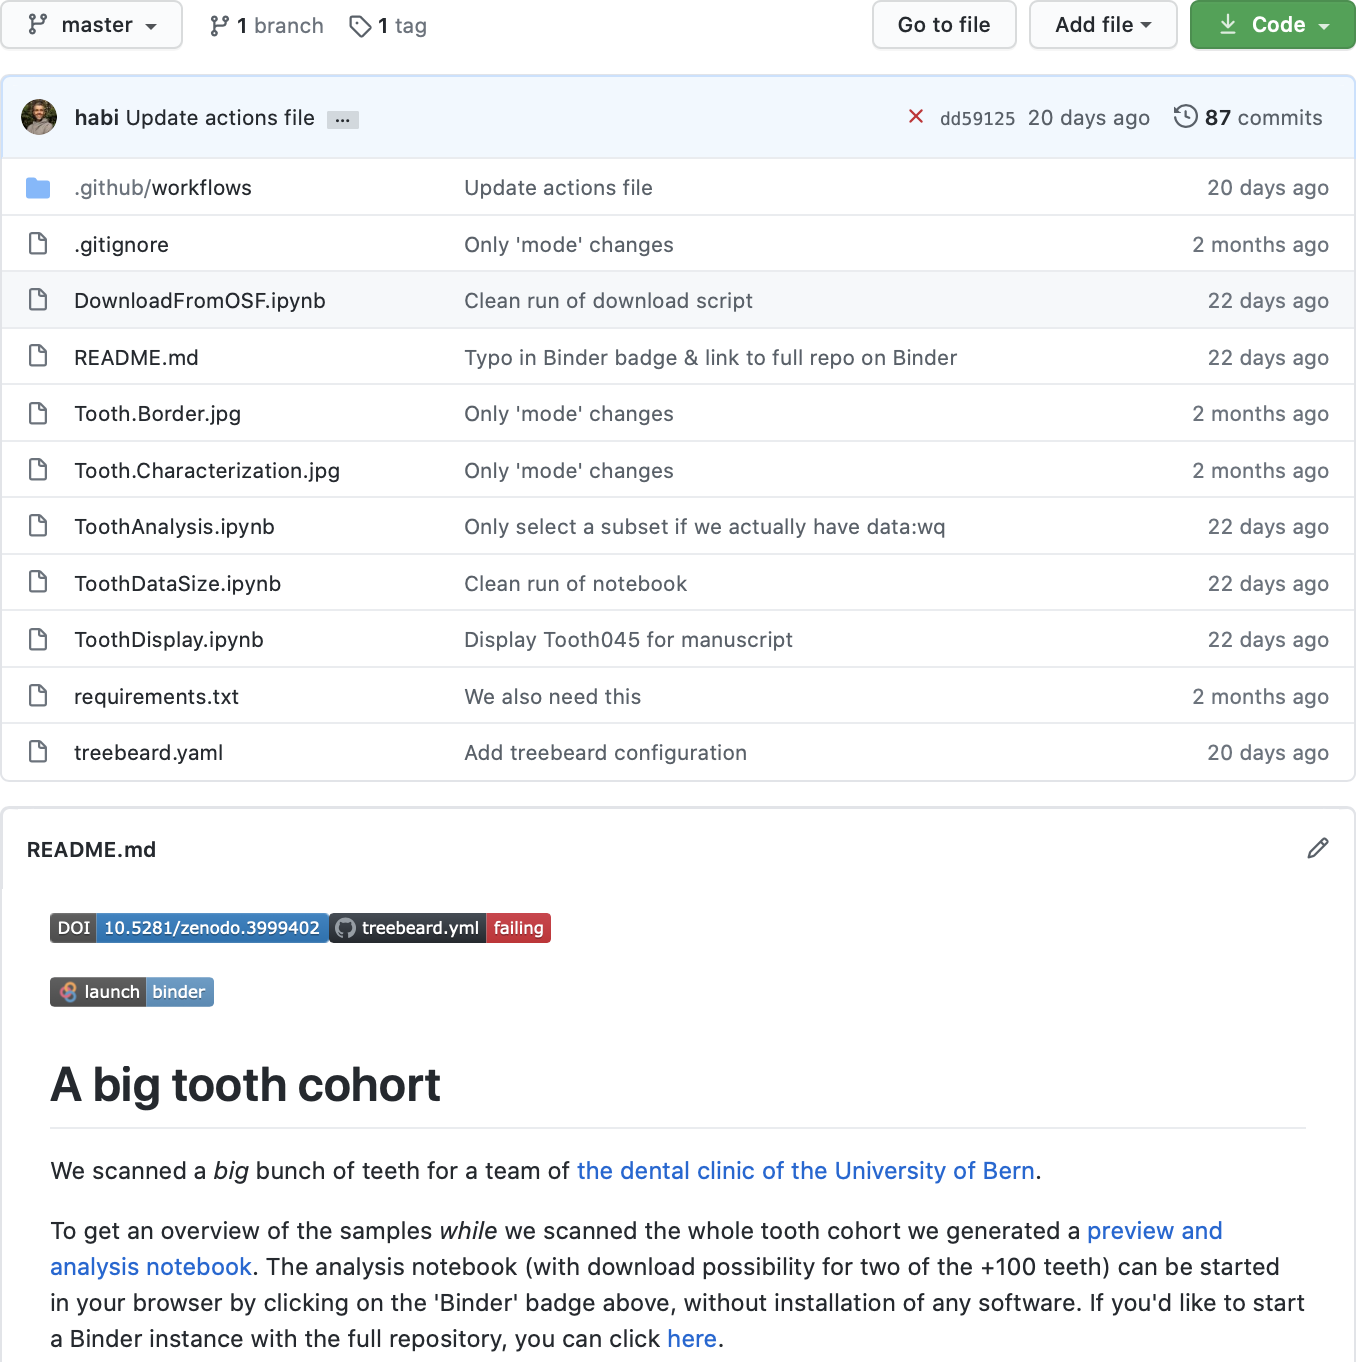
\includegraphics[height=\imheight]{./images/binder}}%
				}%
		\end{column}%
	\end{columns}%
\end{frame}

\begin{frame}
	\frametitle{Tooth morphology}
	% python ~/Dev/latex/draw_a_scalebar.py -p 9.999986 -l 2404 -i images/ZMK/tooth045/full/image0000.png
	\begin{tikzpicture}[remember picture,overlay]%
		\node at (current page.center) [shift={(0,-25pt)}]{%
			\only<1>{
			\tikzset{shadowed/.style={preaction={transform canvas={shift={(1pt,-1pt)}},draw=ubRed, thick}}} % shadowed drawing https://tex.stackexchange.com/a/185853/828
\pgfmathsetlength{\imagewidth}{\paperwidth}%
\pgfmathsetlength{\imagescale}{\imagewidth/1024}%
\def\x{633}% scalebar-x starting at golden ratio of image width of 1024px = 633
\def\y{323}% scalebar-y at 90% of image height of 359px = 323
\begin{tikzpicture}[x=\imagescale,y=-\imagescale]
		\node[anchor=north west, inner sep=0pt, outer sep=0pt] at (0,0) {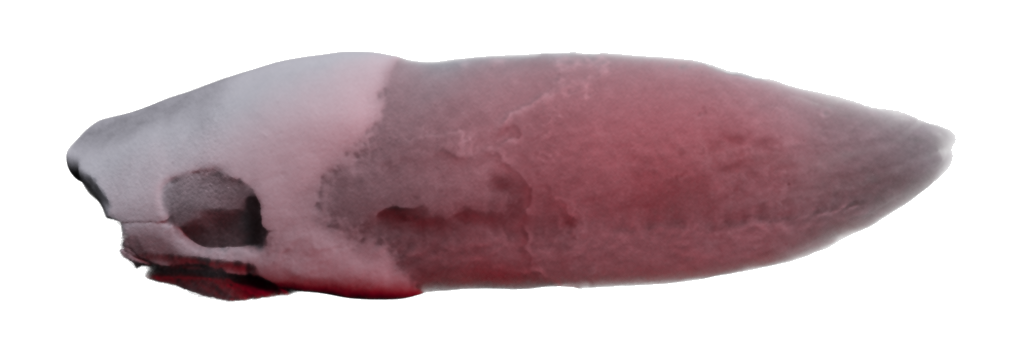
\includegraphics[width=\imagewidth]{./images/ZMK/45/full/image0001}};
	% 881.723px = 24.039966344mm -> 100px = 2726.476um -> 18.339px = 500um, 3.668px = 100um
	%\draw[|-|,blue,thick] (69,158) -- (950,140) node [sloped,midway,above,fill=white,semitransparent,text opacity=1] {\SI{24}{\milli\meter} (882px) TEMPORARY!};
	\draw[|-|,white,thick,shadowed] (\x,\y) -- (\x+183.39,\y) node [midway,above] {\shadowtext{\SI{5}{\milli\meter}}};
\end{tikzpicture}%
			}%
			\only<2>{\animategraphics[autoplay,loop,width=\paperwidth,every=\everyframe]{24}{./images/ZMK/45/full/image0}{001}{238}}%
			\only<3>{\animategraphics[autoplay,loop,width=\paperwidth,every=\everyframe]{24}{./images/ZMK/45/full-slices/image0}{001}{234}}%
			};%
	\end{tikzpicture}%
\end{frame}

\begin{frame}
	\frametitle{Tooth morphology}
	\begin{tikzpicture}[remember picture,overlay]%
		\node at (current page.center) [shift={(0,-25pt)}]{%
			\only<1>{\animategraphics[autoplay,loop,width=\paperwidth,every=\everyframe]{24}{./images/ZMK/45/transparent-slices/image0}{001}{237}}%	
			\only<2>{\animategraphics[autoplay,loop,width=\paperwidth,every=\everyframe]{24}{./images/ZMK/45/transparent-slices-pulpa/image0}{001}{229}}%
			};%
	\end{tikzpicture}%
\end{frame}

\begin{frame}
	\frametitle{Meteorite Chondrules}
	\begin{columns}
		\begin{column}{0.495\linewidth}
			\begin{itemize}
				\item Space Research \& Planetary Sciences
				\begin{itemize}%
					\item Yogita Kadlag
					\item Ingo Leya
				\end{itemize}
				\item Chondrules from outer space
				\item Quantifying physical and chemical properties
			\end{itemize}
		\end{column}
		\begin{column}{0.495\linewidth}
\lstinputlisting[linerange={2-4,7-7,15-18,28-29,31-31,37-38,42-42,46-46,57-58},linebackgroundcolor={\ifnum\value{lstnumber}=11\color{ubRed!31}\fi}]{./images/"Chondrules Space Yogita"/NWA1241_HR2/proj/NWA1241.log}%
		\end{column}
	\end{columns}
\end{frame}

\begin{frame}
	\frametitle{Meteorite Chondrules}
	% Scaled Image Pixel Size (um)=0.399990
	% We used a binned dataset for the visualisation, e.g. the voxel size is 0.79998 um
	% The diameter of the chondrule is ~1263 voxels, so we used `python ~/P/Dev/latex/draw_a_scalebar.py -p 0.79998 -i frames/video-0000.jpg -l 1236` to generate a scale bar for both views.
	\renewcommand{\imheight}{0.618\paperheight}%
	\renewcommand{\imwidth}{\imheight}% The image is square, so we just reuse this.
	\centering%
		\tikzset{shadowed/.style={preaction={transform canvas={shift={(1pt,-1pt)}},draw=ubRed, thick}}} % shadowed drawing https://tex.stackexchange.com/a/185853/828
		\pgfmathsetlength{\imagewidth}{\imwidth}%
		\pgfmathsetlength{\imagescale}{\imagewidth/1024}%
		\def\x{633}% scalebar-x starting at golden ratio of image width of 1024px = 633
		\def\y{922}% scalebar-y at 90% of image height of 1024px = 922
		\only<1>{%
			\begin{tikzpicture}[x=\imagescale,y=-\imagescale]
				\node[anchor=north west, inner sep=0pt, outer sep=0pt] at (0,0) {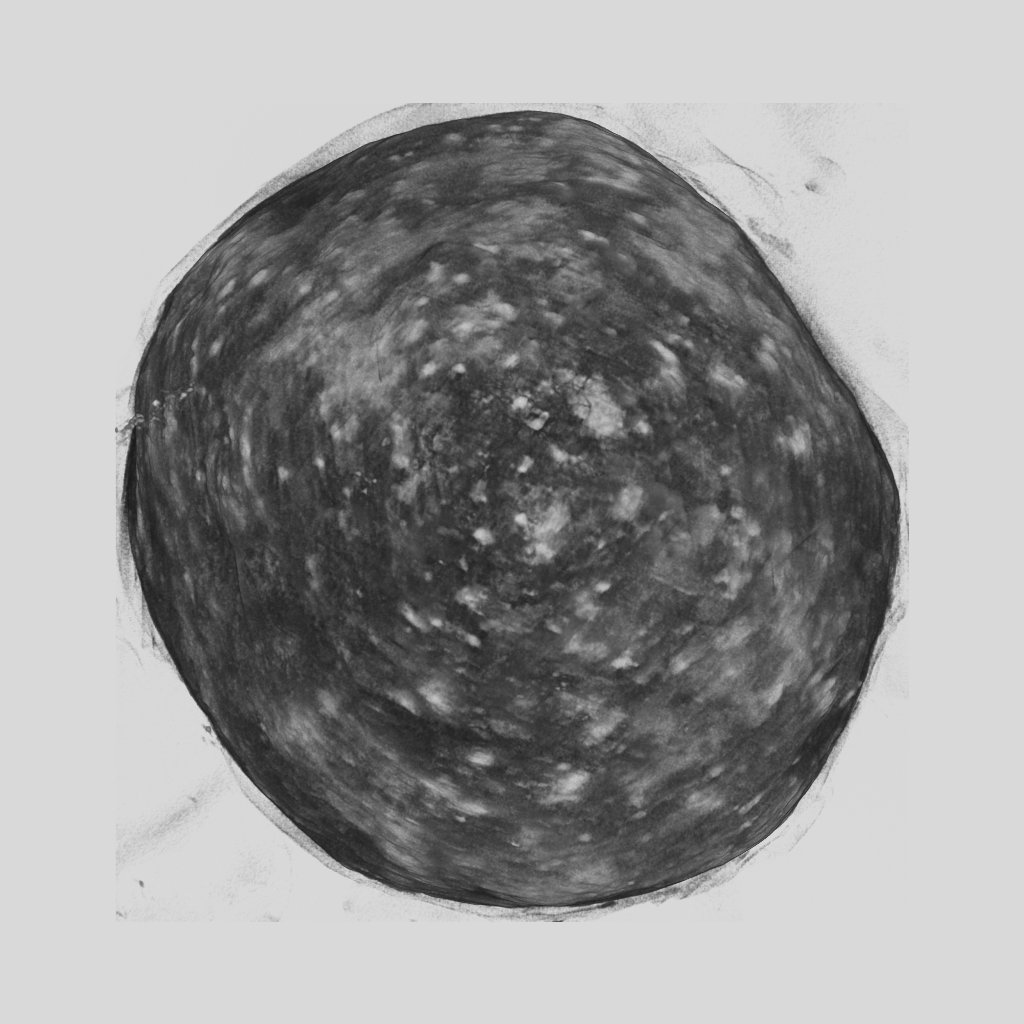
\includegraphics[width=\imagewidth]{./images/Chondrules Space Yogita/NWA1241_HR2/frames/video-0000}};
				% 49.947px = 0.98877528mm -> 100px = 1979.648um -> 25.257px = 500um, 5.051px = 100um
				%\draw[|-|,blue,thick] (489,516) -- (539,513) node [sloped,midway,above,fill=white,semitransparent,text opacity=1] {\SI{0.98877528}{\milli\meter} (50px) TEMPORARY!};
				\draw[|-|,white,thick,shadowed] (\x,\y) -- (\x+25.257,\y) node [midway,above] {\shadowtext{\SI{500}{\micro\meter}}};
			\end{tikzpicture}%
		}%
		\only<2>{%
			\animategraphics[autoplay,height=\imheight,every=\everyframe]{24}{./images/"Chondrules Space Yogita"/NWA1241_HR2/frames/video-0}{000}{100}
		}%
		\only<3>{%
			\begin{tikzpicture}[x=\imagescale,y=-\imagescale]
				\node[anchor=north west, inner sep=0pt, outer sep=0pt] at (0,0) {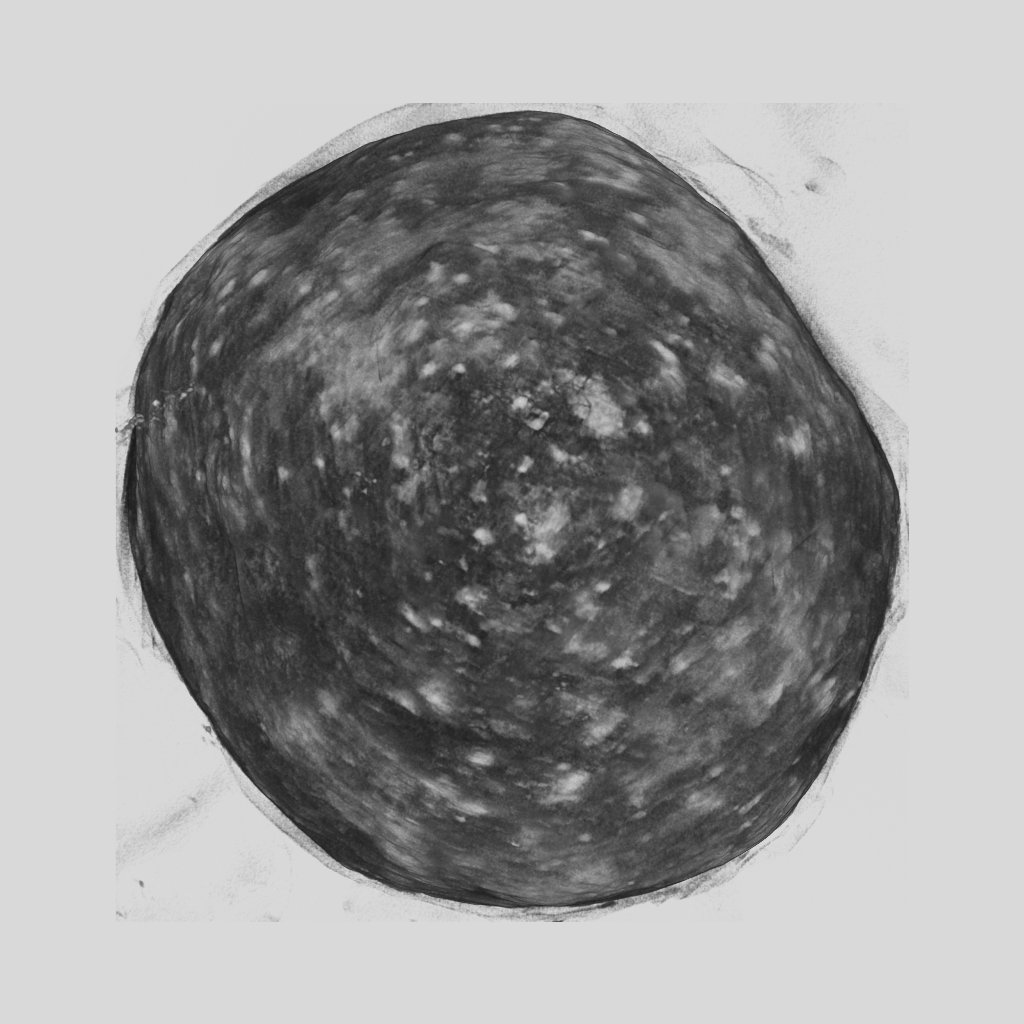
\includegraphics[width=\imagewidth]{./images/Chondrules Space Yogita/NWA1241_HR2/frames/video-0100}};
			% 867.722px = 0.98877528mm -> 100px = 113.951um -> 438.786px = 500um, 87.757px = 100um
			%\draw[|-|,blue,thick] (79,497) -- (946,527) node [sloped,midway,above,fill=white,semitransparent,text opacity=1] {\SI{0.98877528}{\milli\meter} (868px) TEMPORARY!};
			\draw[|-|,white,thick,shadowed] (\x,\y) -- (\x+438.786,\y) node [midway,above] {\shadowtext{\SI{500}{\micro\meter}}};
		\end{tikzpicture}
		}%
		\only<4>{%
			\animategraphics[autoplay,height=\imheight,every=\everyframe]{24}{./images/"Chondrules Space Yogita"/NWA1241_HR2/frames/video-0}{100}{350}%
			}%
\end{frame}

\begin{frame}[label=current]
	\frametitle{Thanks}
	\begin{columns}
		\begin{column}{0.495\linewidth}
			\begin{itemize}
				\item All the collaborators, for collaborating
				\item SNF, for paying my wages
				\item<2-> You, for listening to me%
			\end{itemize}%
	\end{column}
	\begin{column}{0.495\linewidth}
		\StickyNote[2.5cm]{\centering \LARGE Sign up for COMULIS\\
			Training School:\\
			\hrefl{bit.ly/uctworkshop}{https://www.ana.unibe.ch/continuing_education/comulis_training_school/index_eng.html}}[6.5cm]
		\end{column}
	\end{columns}
\end{frame}

\begin{frame}
	\frametitle{References}
	% Make the references continuously smaller :)
	%\renewcommand*{\bibfont}{\small}
	%\renewcommand*{\bibfont}{\footnotesize}
	%\renewcommand*{\bibfont}{\scriptsize}
	%\renewcommand*{\bibfont}{\tiny}
%	\setbeamertemplate{bibliography item}{\insertbiblabel}
	\printbibliography
\end{frame}

\end{document}
